\chapter{Интеллектуальных анализ данных Web-ресурсов}\label{ch:ch5}

\section{Анализ Web-графов}\label{sec:ch5/sect1}

\subsection{Beyond left and right: Real-world political polarization in twitter discussions on inter-ethnic conflicts}\label{subsec:ch5/sec1/sub1}

\subsection{Please Follow Us: Media roles in Twitter discussions in the United States, Germany, France, and Russia}\label{subsec:ch5/sec1/sub2}

\subsection{Multi-dimensional echo chambers: Language and sentiment structure of Twitter discussions on the Charlie Hebdo case}\label{subsec:ch5/sec1/sub3}

\subsubsection{1. Introduction}

Public discussions on social networks potentially have trans-border and multilingual nature. This comes true in heated conflictual discussions that reach global trending topics. Such discussions are expected to demonstrate ‘civilizational clashes’ \cite{AnKwakMejova}.

Being part of the global public sphere, since the 1990s, such discussions were expected by many observers to be more horizontal, all-involving, and democratically efficient \cite{Fuchs} than the traditional mass-mediated discussions \cite{McQuail}. But, with time, criticism towards the democratic quality of discussions in social media arose, with many works discovering the patterns of echo chambering and discourse polarization in social networks \cite{Sunstein2001,Sunstein2002,BarberaJostNagler,BastosMerceaBaronchelli,ColleoniRozzaArvidsson,ConoverRatkiewiczFrancisco}, which lowered the capacities of inter-group discussions and, thus, just formed an additional line of social segregation.

Object-oriented hashtagged discussions have been thoroughly studied in the 2010s, including those on political and social conflicts. But there is still scarce knowledge on whether affective hashtags \cite{Papacharissi} that convey emotions -- either of solidarity with or of anger towards a particular social group -- work in terms of user clusterization. Also, there is no clear understanding of comparative democratic quality of emotionally ‘positive’ and ‘negative’ hashtags in terms of echo chambering.

In this paper, we address these gaps by analyzing the Twitter discussion on the \textit{Charlie Hebdo} massacre of 2015. In the discussion upon the mass killings, the Twittershpere has created \#jesuischarlie and \#jenesuispascharlie -- two emotionally differing discussion clusters with, allegedly, opposite sentiments towards the journal’s ethics and freedom of speech; the hashtags soon became ‘role models’ for online solidarity towards the victims of terrorist attacks and anthropogenic disasters.

To analyze the echo chambering patterns in the two discussions, we have focused upon two levels of echo chambers. We were wondering whether echo chambers formed on the level of a hashtag (based on language use) and within a particular language (based on user sentiment of French-speaking users).
The remainder of the paper is organized as follows. Section 2 reviews the literature on echo chambering in social media. Section 3 presents our methodology and the conduct of the research. Section 4 presents our results and discusses them.

\subsubsection{2. User Groupings on Twitter and the Efficacy of Public Sphere}

\paragraph{2.1 Social Media and the Public Sphere: Echo Chambers vs. Opinion Crossroads}
Public sphere as a spatial metaphor for a complex of discussions and procedures with a public status and decision-making goals \cite{Kleinstuber} has been amplified by the appearance of social media in the 2000s. By 1990s, it had been established in the academic literature that mediatized public sphere with traditional media playing the role of information hubs was uneven and hardly efficient in terms of access to opinion expression, as whole social groups remained under-represented, and newsmakers privileged in comparison to \textit{vox populi}. With the appearance of social media, hopes arose that the new communicative milieus would foster horizontalization of communication and provide for democratization and higher political participation \cite{Fuchs}. Also, hopes for better understanding and resolution of non-political inter-group conflicts existed.

But with time, these hopes fainted, as offline disparities seemed to reproduce online, including political interests, race, gender, and other inequalities \cite{Daniels}; emotion and affect proved to rule the discourse \cite{Papacharissi}, with publics even in most democratically developed countries moving from diverse in opinion to dissonant and disconnected \cite{Pfetsch}. With the development of social network analysis (SNA) and its application to social media research, the question of the efficacy of the public discussions in social media \cite{BrunsHighfield} became linked to network and structural features of the discussions, such as the influencer status \cite{BodrunovaBlekanovMaksimov,BodrunovaLitvinenkoBlekanov2016} and clusterization of users also known as user polarization \cite{BarberaJostNagler,BastosMerceaBaronchelli} and echo chambering \cite{ColleoniRozzaArvidsson,ConoverRatkiewiczFrancisco}. Some evidence was also gathered on discussion sphericules forming on the global scale just as well as nationally \cite{CammaertsAudenhove}.

\paragraph{2.2 Why the Twitter Discussions Fragment: Linguistic Properties of Speech as Catalyzers of Echo Chambering}
In early studies of social networks and its users, authors interested in testing the ability of networks to pull together users from distant locations and weak ties linked geo- graphical distance with factors like residence of users and their language profile \cite{TakhteyevGruzdWellman}. This is why Twitter that enabled the (arguably) quickest possible information spread across locations and languages became a major attractor of scholarly attention \cite{LotanGraeffAnanny,HongConvertinoChi}. But despite the global reach of the platform, several studies have found that people were still connected locally on Twitter \cite{CammaertsAudenhove,YardiBoyd}.

Along with locality and residence, linguistic factors, arguably, play a major role in user grouping on the global scale. Thus, the language(s) used by the discussion participants is the first natural barrier that is expected to make users group together and communicate within their language-based echo chambers \cite{ChenTuZheng}, both on Twitter on the whole and within particular hashtags \cite{BastosPuschmannTravitzki}.

Other factors have also been discussed as the catalyzers of user grouping on Twitter. Among those, political attitudes lead the research agenda \cite{BarberaJostNagler,BastosMerceaBaronchelli}. Here, several ways to detect user clusterization exist. Of them, use of network or semantic proxies like friendship ties \cite{BarberaRivero}, patterns of following \cite{Rivero} and retweeting \cite{CalaisGuerraMeiraJrCardie}, content sharing \cite{ColleoniRozzaArvidsson,BakshyMessingAdamic} etc. is till today the most prominent; another is automated analysis of user sentiment, either in general or toward an issue/actor in question (object-oriented) \cite{ConoverGoncalvesRatkiewicz}.

But all these studies depict user groupings within a single dimension; our idea is to try and trace user groupings multi-dimensionally -- both on the level of a hashtag (based on language use) and within a language nebula (based on user sentiment).

\paragraph{2.3 The \textit{Charlie Hebdo} Case: Emotional Hashtags and User Groupings}
To search for multi-dimensional echo chambers, we have chosen the case of the \textit{Charlie Hebdo} massacre of 2015. Here, we could hypothesize that the existence of emotionally opposite hashtags (\#jesuischarlie and \#jenesuispascharlie) already creates enclaves within the general discussion on the case. Then, within the hashtags, several clusters based on language structure may exist. Then, on the third level, we will look whether within the language clusters sub-clusters of sentiment form. In general, our idea is to see how exactly the language clusters correspond to the sentiment clusters in each language and whether ‘positive’ users within one language are linked to such in another language, while ‘negative’ users also group across languages in a similar way. But here we present only preliminary results that check if the user clusters may at all be detected based on language and on sentiment within a language.

\paragraph{2.4 Research Hypotheses}

Thus, our hypotheses are the following:
\begin{itemize}
	\item H1a. Non-random user groups will be detected for both hashtags, as based on
	language use.
	\item H1b. \#jesuischarie will not differ from \#jenesuispascharlie in their language
	structure, as both hashtags have reached global trending topics and are expected to show ‘civilizational clashes’.
	\item H2a. Non-random user groups will be detected within one language (French), as based on positive and negative sentiment.
	\item H2b. \#jesuischarlie will differ from \#jenesuispascharlie in the grouping based on user sentiment, due to the emotional opposition of the hashtags themselves.
	\item H3. Multi-layer echo chambering may be detected in trans-border hashtagged discussions of global reach.
\end{itemize}

\subsubsection{3. Data Collection and Conduct of Research}

\paragraph{3.1 Data Collection and the Datasets}
Using a web crawler developed especially for the Twitter data collection, we gathered all the tweets published openly under the hashtags \#jesuischarlie and \#jenesuispascharlie (by separate crawls) within January 7 to 9, 2015, as these three days covered the active conflict (from the killings in the editorial office to the assailants’ death) when the users provided virtually millions of tweets for collection.

The collected datasets included: for \#jesuischarlie: 420,080 tweets; 266,904 tweeters; 719,503 users who interacted with the posted tweets (by likes, retweets, or comments); for \#jenesuispascharlie: 7,698 tweets; 5,466 tweeters; 17,872 users who posted and interacted with the posted tweets (by likes, retweets, or comments).

These full datasets were later used to reconstruct the overall web graphs for the two hashtags. But the datasets were very different in size, and be able to color them with language markers, we needed to sample the users for coding having in mind the volume difference of the datasets.

\paragraph{3.2 Language Analysis: Sampling, Coding, and Graph Reconstruction} 
To answer H1a and H1b, we have coded the users for their language use and then applied these data to the datasets for web graph reconstruction.

After eliminating bots and bot-like users (those who posted over 60\% of doubled tweets) as well as hashtag-only tweets, we have followed the strategy developed by the research group for previous Twitter studies \cite{Authors2016a,Authors2016b,Authors2018}, namely uniting random sampling with detection of influential users (influencers) for taking them into account. Then, we have coded all the influencers (disregarding the number of tweets they posted; for \#jesuiuscharlie, 402 users, for \#jenesuispascharlie, 85 users) and ‘ordinary users’ sampled in the feasible and comparable way. For \#jenesuispascharlie that was substantially smaller, all the users with 3 and more tweets were coded (339 users); for \#jesuischarlie, the ‘ordinary users’ with 5 tweets or more were taken into account (9,090 users), and of them, each second was coded (4500 users).

All the sampled underwent expert reading and were coded manually marking the number of tweets in language 1, language 2, and other languages; thus, users posting on one, two, and three or more languages were defined. The languages were identified for each user; in case of rare languages, Yandex language identifier was employed.

To reconstruct the graphs, we use Gephi API algorithms openly available online. Of the available algorithms, two were chosen: Hu \cite{Hu} and OpenOrd \cite{MartinBrownKlavans}; here, YifanHu-based graphs are presented, as the OpenOrd graphs require more space for presentation. We colored both the nodes (users) and the edges (connections between users). To prove that the visual nebulae are not artifacts of subjective viewership, we calculated the percentage of edges between and inside language groups, eliminating the ‘loops’ of self-commenting/liking by the users.

\paragraph{3.3 Sentiment Analysis: Sampling, Vocabulary Building, and Graph Reconstruction}After we have proved that the French-speaking users show non-random grouping in both cases (see below), we have taken them for sentiment analysis. The number of users for \#jesuischarlie included 1291 user; for \#jenesuispascharlie, 117 users.

Our strategy for French-language sentiment analysis was the following. We have united three sources in our vocabulary: the existing French dictionary with sentiment marking, machine translation from an additional Wordnet vocabulary, and the case-based vocabulary created from the collected tweets and manually marked for positive, negative, and neutral sentiment regardless of the case-specific meanings.

This vocabulary was applied to each tweet of the abovementioned French-speaking users; for each tweet, the sentiment was calculated. Then, the thresholds were defined: positive and negative were the users with positive(+neutral) and negative(+neutral) tweets, respectively; neutral were those with neutral tweets only; mixed were those with positive + negative(+neutral) tweets.

Then, we also checked the groupings with by calculating the percentage of edges both between and inside language groups, eliminating the ‘loops’ of self-commenting/liking by the users.

\subsubsection{4. Results and Discussion}

Our results are described below with regard to the hypotheses stated above.

\textit{H1a/H1b.} To assess the user groupings in both hashtagged discussions, we have reconstructed the web graphs for the coded users (see Fig.~\cref{fig:yifanHuGraphs-2} for \#jesuischarlie and Fig.~\cref{fig:yifanHuGraphs-2} for \#jenesuispascharlie, respectively). What we see on the graphs are three nebulae for~\cref{fig:yifanHuGraphs-1}: French, English, and other European, and two for~\cref{fig:yifanHuGraphs-2}: French and Engish. But the results of calculations of percentage of edges between and inside groups tell that the actual grouping is slightly different from what we see with unaided eyes. For \#jesuischarlie, the nebulae with density higher than the inter-group ones are French, English, and French/English (52.1\%, 16.7\%, and 16.9\%, respectively, against 6.17\% for inter-group edges) and not other European. For \#jenesuispascharlie, the graph is much denser (26\%), but still the same three clusters show up, with 26.2\%, 22.4\%, and 18.8\%, respectively; in both cases, other language clusters are virtually non-existent and do not mount to 3\%. As we stated in our earlier investigations \cite{Authors2018}, we have not seen a sign of ‘civilizational clashes’ in any of the hashtags.

\begin{figure}[ht]
	\centerfloat{
		\hfill
		\subcaptionbox[List-of-Figures entry]{\label{fig:yifanHuGraphs-1}}{%
			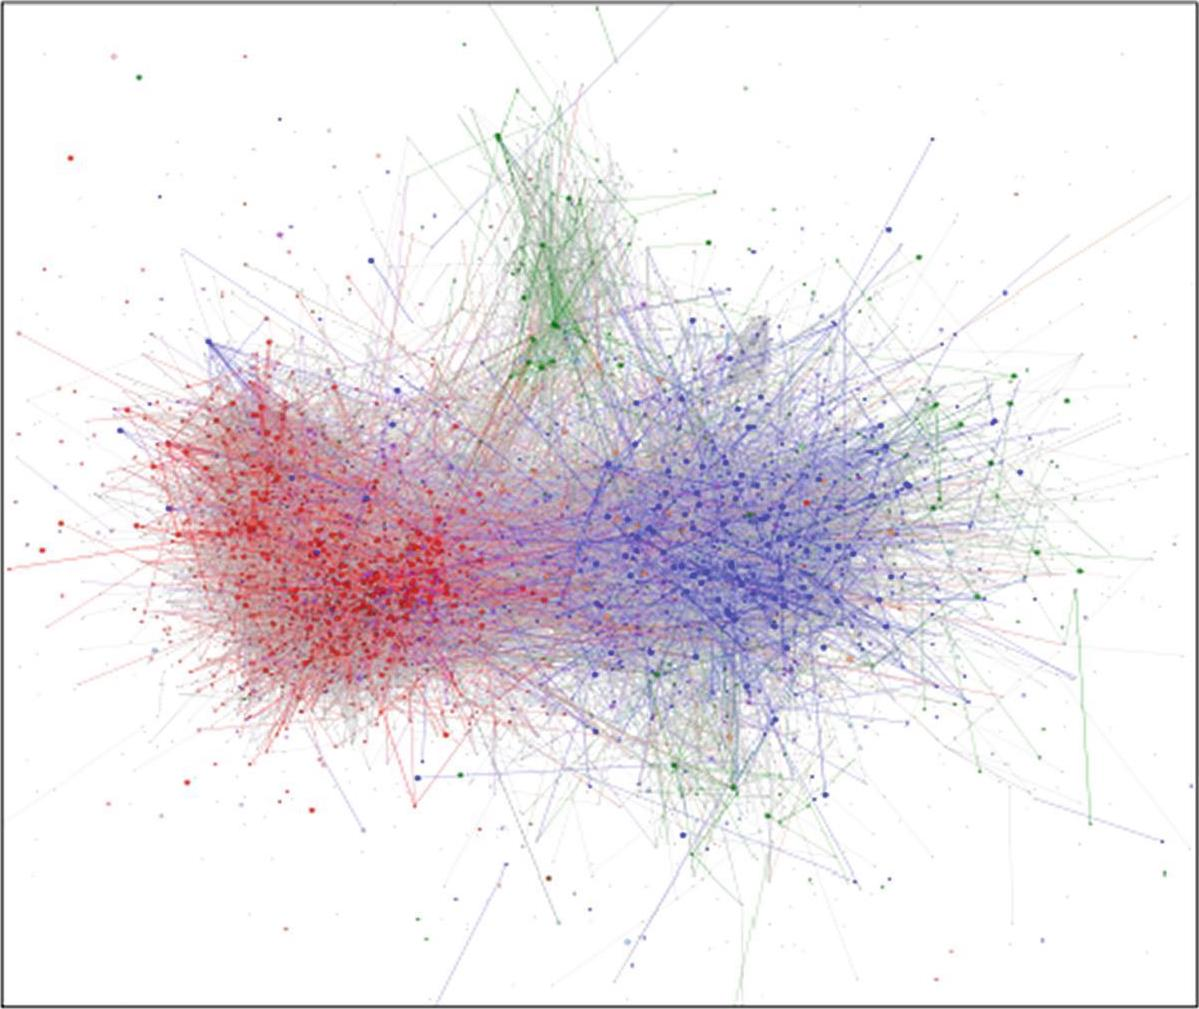
\includegraphics[width=0.419\linewidth]{yifanHuGraphs1}}
		\subcaptionbox{\label{fig:yifanHuGraphs-2}}{%
			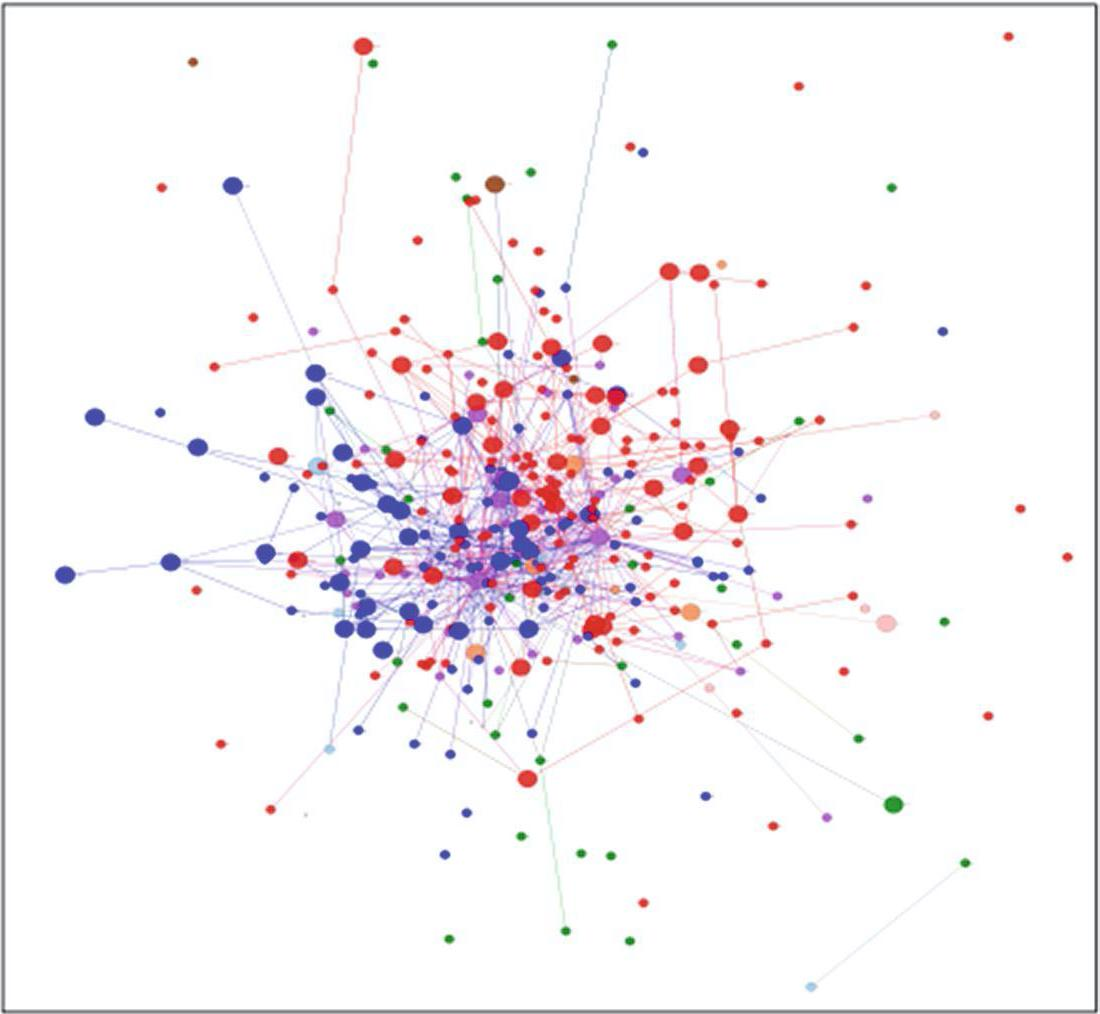
\includegraphics[width=0.4\linewidth]{yifanHuGraphs2}}
		\hfill
	}
	\caption{The YifanHu graphs (fragments) for language distribution in \cref{fig:yifanHuGraphs-1} \#jesuischarlie and \cref{fig:yifanHuGraphs-2} \#jenesuispascharlie. Red: French; blue: English; lilac: French/English; green: other European. (Color figure online)}\label{fig:yifanHuGraphs-12}
\end{figure}

Thus, H1a is proven; H1b is proven too but not due to ‘civilizational clashes’.

\textit{H2a/H2b.} To see the user grouping and sentiment cleavages within the French-speaking parts of the discussions, we have reconstructed the web graphs for them (see Fig.~\cref{fig:yifanHuGraphs-3} for \#jesuischarlie and Fig.~\cref{fig:yifanHuGraphs-4} for \#jenesuispascharlie, respectively).

\begin{figure}[ht]
	\centerfloat{
		\hfill
		\subcaptionbox[List-of-Figures entry]{\label{fig:yifanHuGraphs-3}}{%
			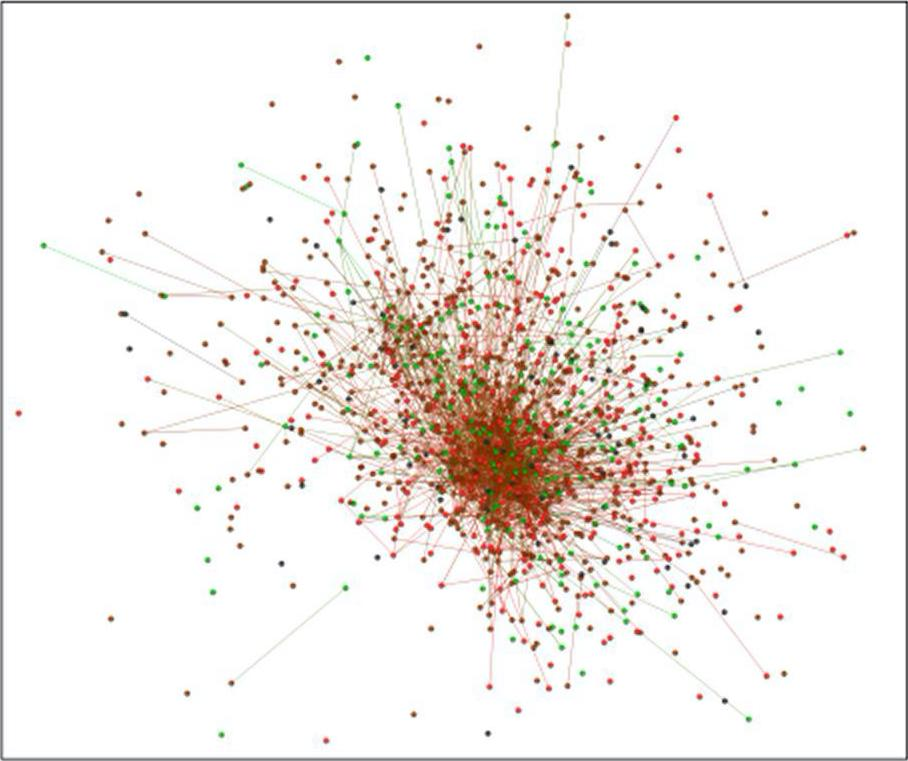
\includegraphics[width=0.419\linewidth]{yifanHuGraphs3}}
		\subcaptionbox{\label{fig:yifanHuGraphs-4}}{%
			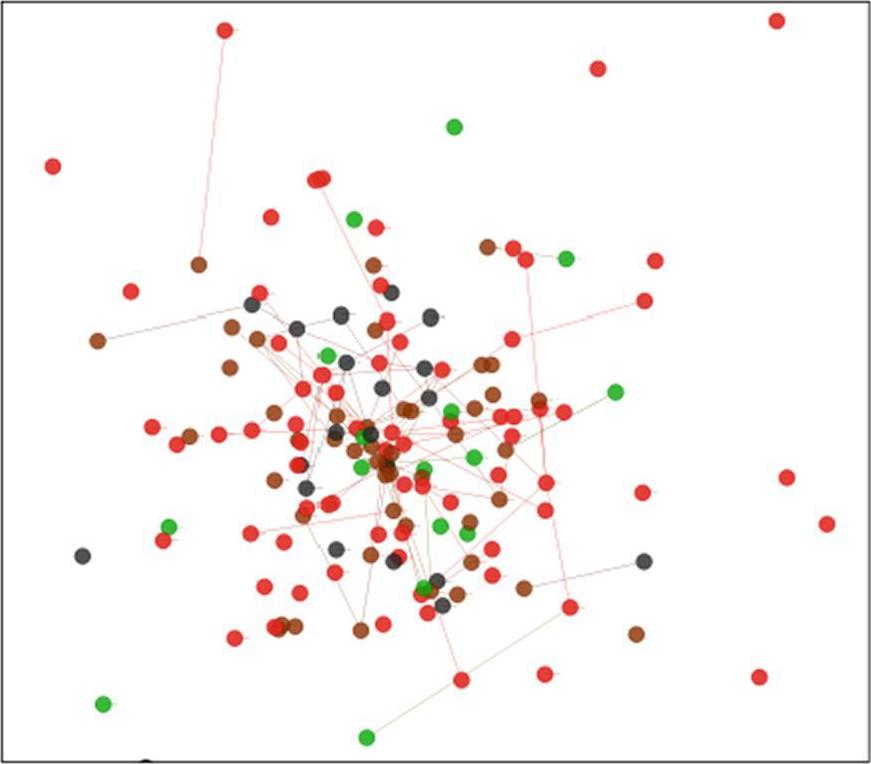
\includegraphics[width=0.4\linewidth]{yifanHuGraphs4}}
		\hfill
	}
	\caption{The YifanHu graphs (fragments) for language distribution in \cref{fig:yifanHuGraphs-3} \#jesuischarlie and \cref{fig:yifanHuGraphs-4} \#jenesuispascharlie. Red: French; blue: English; lilac: French/English; green: other European. (Color figure online)}\label{fig:yifanHuGraphs-34}
\end{figure}

Here, H2a should be rejected for \#jesuischarlie and partly supported for the second hashtag. Both in the graph and in the edge percentage calculations, it is only users with mixed sentiment who form a group (38.33\% against 56.05\% for the inter-group connections) in \#jesuischarlie. But for \#jenesuispascharlie, both mixed and negative user groups seem to have a potential for grouping (19.5\% and 15\% against 62.1\% for inter-group connections). Thus, H2b is supported: the cases do differ.

Even with the cases of such different sizes, H3 is supported: thanks to the negative nebula in \#jenesuispascharlie, we can state that echo chambers are able to form on at least two levels of the trans-border conflictual discussions of global (or, more precisely, macro-regional) reach. This adds to our understanding of the nature of public discussions in social media, even if lowers hopes for all-encompassing public spheres.

\section{Тематическое моделирование контента}\label{sec:ch5/sect2}

\section{Методы анализа тональности контента}\label{sec:ch5/sect3}

\section{Методы суммаризации}\label{sec:ch5/sect4}

\FloatBarrier

